\chapter{Architettura Pulita}
\begin{boxDef}
\textbf{\textcolor{brown}{Obiettivo:}} creare un'architettura per massimizzare la produttività dividendola in componenti che comunicano. \\
\textbf{\textcolor{brown}{Scopo:}} facilitare comprensibilità, sviluppo, distribuzione, operatività e mantenimento quindi supportando l'intero ciclo di vita lasciando opzioni aperte.

\begin{itemize}
    \item \textbf{Sviluppo:} un software che ha uno sviluppo difficile non avrà vita lunga.
    \item \textbf{Distribuzione:} un software che è costoso da distribuire e compilare sarà poco utile.
    \item \textbf{Operatività:} non è molto influenzata all'architettura perché c'entra l'hardware ma dovrebbero Sfruttarla per renderle leggibili allo sviluppatore.
    \item \textbf{Mantenimento:} il costo principale del mantenimento è la \textit{speleologia}, ossia cercare dove aggiungere nuove funzioni, e il rischio di rompere tutto.
\end{itemize}
\end{boxDef}
\begin{itemize}
    \item \textbf{\textcolor{brown}{Disaccoppiamento dei livelli:}} si usano \textbf{SRP} e \textbf{CCP} separando la gestione UI, dalle regole di business dipendenti (e non) dall'applicativo e il livello del DB.
    \item \textbf{\textcolor{brown}{Disaccoppiamento use-case:}} si tratta di creare fette verticali sui livelli, in modo da separare porzioni di codice che cambiano in base alla funzionalità.
\end{itemize}

\section{Livelli di Disaccoppiamento}
\begin{enumerate}
    \item \textbf{\textcolor{brown}{Livello sorgente:}} pone l'attenzione sull'evitare dipendenze nei moduli centrali in modo da evitare di ricompilarli tutti per ogni modifica.
    \item \textbf{\textcolor{brown}{Livello di distribuzione:}} pone l'attenzione sull'evitare dipendenza tra unità distribuibili che devono essere indipendenti l'un l'altra.
    \begin{enumerate}
        \item I componenti risiedono nello stesso spazio indirizzi e utilizzano chiamate a funzioni, comunicando con \textbf{IPC}, \textbf{socket} o \textbf{memoria condivisa}.
    \end{enumerate}
    \item \textbf{\textcolor{brown}{Livello servizi:}} le dipendenze sono ridotte alla comunicazione livello dati, mentre i componenti comunicano tramite pacchetti rete e sono indipendenti.
    \begin{enumerate}
        \item Quest'ultimo è tendenzialmente costoso, per cui si inizia da un \textbf{monolite}, poi si divide in \textbf{unità} distribuibili e si espandono in \textbf{servizi} o \textbf{microservizi}.
    \end{enumerate}
\end{enumerate}

È importante tracciare \textbf{confini} per decidere quali componenti sanno dell'esistenza altrui o dipendono da essi, ma le decisioni non devono essere premature. 

\begin{boxDef}
\textbf{\textcolor{red}{Policy:}} regole per trasformare gli input in output che possono essere suddivise in calcoli, formattazione e validazione input. \\
\textbf{\textcolor{red}{Livello:}} la distanza tra gli input e gli output. \\
\textbf{\textcolor{red}{Regole di buisness:}} procedure che esistono al di là della loro digitalizzazione e possono essere critiche per il business usando dati critici. \\
\textbf{\textcolor{red}{Entità:}} oggetti che nascono dai legami intrinseci tra le regole critiche e i loro relativi dati.
\end{boxDef}

\section{Architettura Pulita}
Ogni cerchio concentrico rappresenta aree diverse del software, quelli interni sono le policy, quelli esterni i meccanismi:

\begin{figure}[!htb]
    \centering
    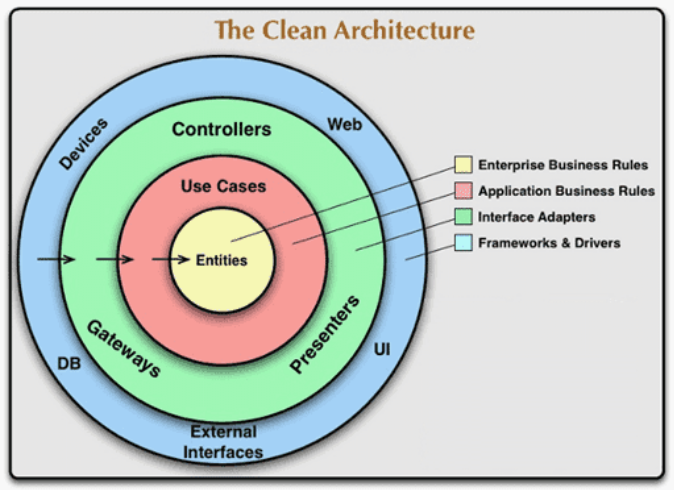
\includegraphics[width=0.5\linewidth]{Images/architettura_pulita/clean.png}
    \caption{Grafico di Architettura Pulita.}
\end{figure}

Dove:
\begin{itemize}
    \item \textbf{\textcolor{brown}{Entità:}} è il cerchio più interno per cui è quello di più alto livello su cui dipende tutto e contiene le regole critiche di business riutilizzabili.
    \item \textbf{\textcolor{brown}{Use-Case:}} cerchio centrale che contiene le regole legate all'applicativo e gestisce il flusso di dati da/a entità e le modifiche qui non toccano le entità.
    \item \textbf{\textcolor{brown}{Interface Adapters:}} converte i dati per passarli ai servizi esterni con adapter, contiene tutti i componenti MVC.
    \item \textbf{\textcolor{brown}{Framework e Driver:}} contiene DB, framework web e altri strumenti e contiene codice minimale che dipende dagli adapters.
    \item \textbf{\textcolor{brown}{Main Component:}} componente più esterno e di basso livello che definisce strategy, factory e utilizza un framework di iniezione delle dipendenze.
\end{itemize}

\section{Documentazione 4+1}
\begin{itemize}
    \item Una vista \textbf{logica} che mostra le astrazioni chiave del sistema.
    \item Una vista di \textbf{processo} che mostra l'interazione in fase run time dei processi.
    \item Una vista di \textbf{sviluppo} che mostra come il software è decomposto per lo sviluppo.
    \item Una vista \textbf{fisica} come il software è distribuito tra i processori dell'hardware.
    \item Documentazione aggiuntiva su altri scenari o use-case. 
\end{itemize}


\section{Modello C4}
\begin{itemize}
    \item \textbf{\textcolor{brown}{System context diagram:}} è una vista che contiene il sistema stesso e le persone che comunicano con esso.
    \item \textbf{\textcolor{brown}{Container diagram:}} contiene tutti i container, come interagiscono tra loro e con le persone.
    \item \textbf{\textcolor{brown}{Component diagram:}} componenti, responsabilità, implementazioni e interazioni di un container.
    \item \textbf{\textcolor{brown}{Code:}} decompone un componente e mostra come è implementato ed è opzionale e sconsigliato.
\end{itemize}

